\documentclass[conference]{IEEEtran}
%\IEEEoverridecommandlockouts
% The preceding line is only needed to identify funding in the first footnote. If that is unneeded, please comment it out.
\usepackage{cite}
\usepackage{amsmath,amssymb,amsfonts}
\usepackage{algorithmic}
\usepackage{graphicx}
\usepackage{textcomp}
\usepackage{xcolor}
\usepackage{hyperref}
\usepackage{caption}
\usepackage{subcaption}
\def\BibTeX{{\rm B\kern-.05em{\sc i\kern-.025em b}\kern-.08em
    T\kern-.1667em\lower.7ex\hbox{E}\kern-.125emX}}

\begin{document}

\title{Performance Analysis Of A Modern Data Store}

\author{\IEEEauthorblockN{Adam CHADER}
\IEEEauthorblockA{\textit{PDS track, Master of Computer Science} \\
\textit{Institut Polytechnique de Paris}\\
Palaiseau, France \\
adam.chader@telecom-paris.fr}
}

\maketitle
\thispagestyle{plain}
\pagestyle{plain}

\begin{abstract}
Nowadays, parallelism is a key aspect of software engineering, and is essential for performant programs. However, concurrent data accesses are a big failing point which can drastically reduce the scalability of a piece of software. Designing parallel software is complicated, and a lot of libraries exist to provide ready-made, optimized data structures for concurrency. However, these libraries seek generalizability, and not efficiency. It has been observed that the entire specification of an object is not necessary for a given program, many only use a few methods that are available, and not all of them. By degrading the specification of objects, to make them perfectly tailored for a specific use case, we can change their implementation and improve performances. We propose applying this concept to a complex, modern data store, Apache Ignite, to figure out whether we can improve its performance without changing a single line of code, but by changing the objects in the libraries used to degraded ones.

\end{abstract}

\begin{IEEEkeywords}
Concurrent programming, parallel programming, performance, databases
\end{IEEEkeywords}

\bigbreak 

\section{Introduction}
This paper is the report of a research project realised for the Parallel And Distributed Systems master at \textit{Institut Polytechnique de Paris}. It describes the work that I realised to apply degradable data structures to Apache Ignite \cite{ignite}, a distributed data store, to improve its performance and scalability.

\subsection{Context}
Up until the beginning of the 21\textsuperscript{st} Century, there had existed a simple rule that could be used to predict the performances of computers. This is known as Moore's Law (Fig.~\ref{moore}). This law states that every two year, the number of transistors doubles on chips. This rule could be used quite flawlessly to predict the speed of software, as there is a direct correlation between the speed of sequential programs and the frequency of CPUs. However, in recent years, several issues have surfaced regarding these assumptions : First, we seem to have reached the minimum physical size of a transistor at around 5 nanometer ; second, the frequency that can be reached by cramming all these transistors in a single CPU core is too high to be dissipated by current means \cite{moore}. As of today, it is extremely complicated and costly to significantly increase the clock speed of a single core. The solution that was found is to put multiple CPU cores in a single machine. The total number of clock cycles per second should continue increasing, while the heat would remain manageable. Intuitively, this solution is perfect : by having two cores instead of one, we could double the total frequency of the CPU, and thus double the speed of software. This is what we call \textit{linear scalability}, and it is still just a dream. There are many reason as to why it is impossible to achieve linear scalability, but they all boil down to the same issue : in order to make the most out of several CPU cores, we need to have them working at the same time. It is possible when the tasks are perfectly parallelizable, but this almost never happens when we want the cores working together. Programs need to access variables in memory, and accessing them in parallel can cause conflicts (we will explain these conflicts in detail later), they also need to access IO which can cause issues. The resulting effect of these issues is that parallel programs often contain sequential portions, where each core has to wait for another core to finish a task. The more sequential portions a parallel program contains, the slower the speedup is. This is described by Amdahl's Law \cite{amdahl} (Fig.~\ref{amdahl}). It describes the speedup of parallelisation as a function of the amount of sequential code.

\begin{figure}[!ht]
\centerline{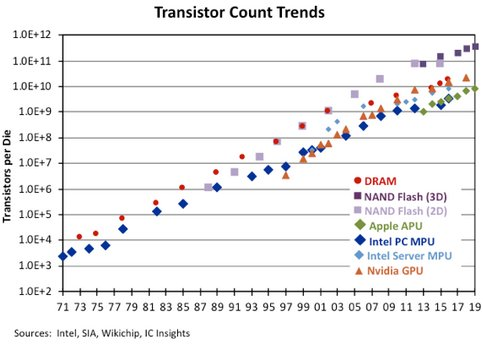
\includegraphics[width=70mm]{moore.jpg}}
\caption{Moore's Law : Every two years, the total number of transistors per chip doubles}\label{moore}
\end{figure}

\begin{figure}[!ht]
\centerline{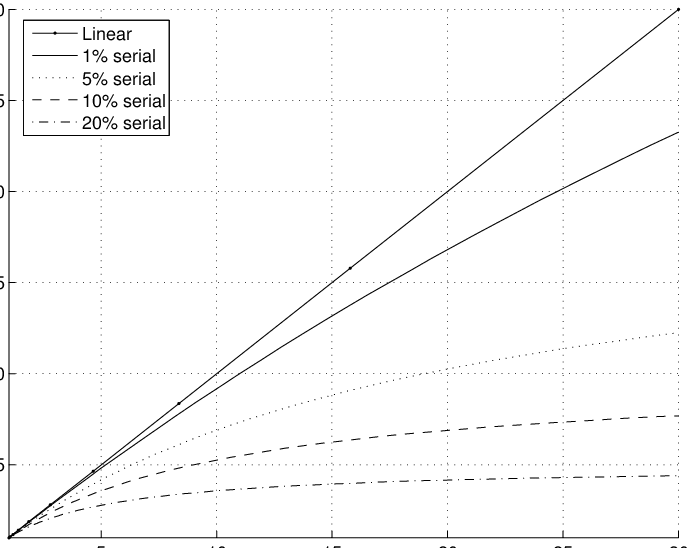
\includegraphics[width=70mm]{amdahl.png}}
\caption{Amdahl's Law : the speedup gained by increasing the number of processors is relative to the amount of sequential code (the serial fraction) of the program.}
\label{amdahl}
\end{figure}

With all of this in mind, it becomes clear that the burden of increasing the performances of software no longer lies in the hands of hardware manufacturers, but rather on the hands of software engineers, who should attempt to have as little sequential code as they can in their programs.
Historically, it was the responsibility of the end programmer to parallelise their program. But there has been work to hide this work in the lower levels of the software stack \cite{scalable}, to make the shift from sequential to parallel transparent to the higher levels. The scope of this work is at a lower level. The goal is to provide perfectly linearly scalable implementations of classic data structures, keeping the exact same interfaces, such that there could be virtually no modification to applications' source, while achieving the scalability that we desire.


\subsection{Work}
This project is a part of a bigger project around \textit{Degradable Data Structures}. These structures will be explained in more detail further in this paper. Simply put, these data structures are created by tweaking the specifications of classical data structures, in order to be able to change their implementations to better ones allowing for better scalability or performance. The idea is to take real industrial code, and change some of the objects used for degraded ones without having to change any of the code, and observe the increase in performance.

\subsection{Scope of this project}
The work being done here is the applications of these degraded data structures to a data store : Apache Ignite \cite{ignite}. We first need to locate situations in the source of the data store where it is judicious to apply degradation. This is done by benchmarking the application, and pinpointing the source of eventual bottlenecks, then figuring out whether or not degradation is possible.

\subsection{Contributions}
This project made the following contributions to Apache Ignite:
\begin{itemize}
  \item Benchmarking
  \item Performance Analysis
  \item Identification of bottlenecks
  \item Method for finding the probable causes of bottlenecks
\end{itemize}

\subsection{Outline}
The rest of this paper details the context and the contributions of the project.

We shall start by examining the related works and how they compare to the work being done here.

We will then explain the theory behind degradable objects and how we can find places to apply them.

We next will detail the information we gathered by analysing Apache Ignite.

we will then show the result obtained.

We will finally discuss the conclusions we can take from the work.

\bigbreak 

\section{Related Work}
\subsection{The Scalable Commutativity rule}
The approach of Austin Clements \cite{scalable} team is very similar to the work being done here. They present a new way of designing scalable and performant software, by thinking on the interface rather than on the implementation. They present the \textit{Scalable Commutativity Rule} that states that \textit{whenever interface operations commute, they can be implemented in a way that scales}. To describe this commutativity they provide a new definition called \textit{SIM-Commutativity} for more complex interfaces. The idea is then to modify the interfaces so that the operations are commutative. This relates very much to the idea of degraded data structures, as they are an extension of this work : rather than saying that the interface needs to be modified, the idea with degradation is to remove some constraints of the previous interface, so that it scales. It could use commutativity or some other form of constraint on the interface.

In the scalable commutativity rule, they work on the interface of the linux kernel, whereas this work is more geared towards data stores and their data structures.

\bigbreak 

\section{Degradable Data Structures}
The goal of this project is to improve the performances of Apache Ignite, by inserting existing degraded data structures \cite{degradation} in the place of traditional ones. We will therefore first explain to what extent the implementation of data structures is linked with performance of parallel applications. We shall then explain the principle behind the degrading of objects, and we will finally explain how we can find the places where it makes sense to apply this degradation.

\subsection{Contention and Scalability} 
The relationship between the implementation of data structures and the performances of parallel applications is not immediate.

To achieve the best performance possible with parallel software, we need for it to scale. Meaning that increasing the number of parallel workers will increase the speed of the computation proportionally. As we have seen with Amdahl's Law, to do this, we need to have as little sequential code as possible in our program. One big source of sequentialness in software is contention in data accesses. Indeed, when two processes try to access and modify the same data point at the same time, the result is non deterministic, which is really bad. To prevent this, safety measures are put in place to prevent concurrent accesses to the same piece of data. Often times, this results in the fact that only one process at a time can access the data, which we will call a \textit{bottleneck}. This introduces sequentialness, and thus we loose in scalability.

We can therefore conclude that the goal of the designer of data structures is to prevent bottlenecks by avoiding contention on the same data points as much as possible, we call this \textit{conflict-freedom}

\subsection{What are Degradable Data Structures ?}
Many libraries provide really performant and scalable implementations of classical data structures for concurrent programming, for example, the Java.Util.Concurrent library \cite{java_concurrent} provides wait-free and linearizable objects. However, the efficiency of these implementations is somewhat limited in a lot of situations, as they are supposed to respect to the letter the specifications (interfaces) of the data structures. Most of the time, these specifications are not designed with performance in mind, rather ease-of-use or generalizability. The goal of the software engineers behind the Concurrent library is not one specific project, rather being able to fit a lot of possible use cases. For example, a classical implementation of a counter needs the increment operation to return the value of the counter. There might be some situations when all these constraints are not necessary, and we loose in performance for nothing.

The idea behind degradation, as described by Boubacar Kane and Pierre Sutra \cite{degradation} is to remove some of the constraints of these specifications when they are not necessary. In the example of the counter for instance, if we say that we do not need for the increment operation to return the value, we can implement the object in such a way that the increment operation only updates a local value to the thread, and we gather the values only when the read operation is called. This would render the increment operation perfectly scalable, and thus really performant.

This is one example of how we can degrade an object, but there are many other solutions, and the work being done right now is to generalize this idea, and formalize it. A key insight is that operations can be implemented with less conflicts, and thus scale more, when their permutation is indistinguishable for future operations. This is an extension of the idea of commutativity from Austin Clements et al. \cite{scalable}. This can be understood quite intuitively : if the order of operations matters little, they can be applied locally and gathered whenever, thus ensuring conflict-freedom.


\subsection{How do we find where to apply degradation ?}
The goal of this project is to apply degradation to a modern, complex software project to see if it can improve performance. To apply them in a way that is significant to performance, we need to locate data structures that are either very important to the whole execution, or that are the cause of a decrease in performance or scalability, \textit{i.e.} bottlenecks. The key question we will try to answer in the rest of this paper is then : How can we identify bottlenecks and their root cause in modern applications ?


\bigbreak 

\section{Performance Analysis of Apache Ignite}
\subsection{Desired Outcome of the analysis}
Ideally, this study will result in the identification of a bottleneck, meaning that increasing the parallel workers of the application no longer results in an increase in performance at some point. Then, we want to be able to locate the root cause of this bottleneck. We ideally want the root cause to be a data structure with a lot of contention, and finally, we would like this data structure to be used by the program in such a way that it is degradable, maybe because not all the methods are used, or because the context of the program is such that there is only one writer or reader. Finally, we would like to see that changing the data structure to a degraded one increases the performances, or even maybe alleviates the bottleneck.

As explained before, we will be working on Apache Ignite, an in-memory data store, where the data is stored in key-value pairs. It is a very complex piece of software, and has over 1.5 million SLOC.


\subsection{Broad benchmarking}

\begin{figure}[!ht]
\centerline{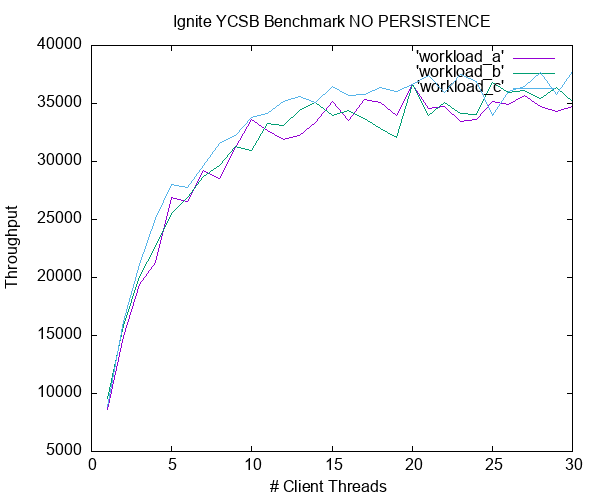
\includegraphics[width=90mm]{coarse_grained.png}}
\caption{YCSB Benchmark on Apache Ignite, while varying the amount of client threads in parallel, three different workloads.}
\label{coarse_grained}
\end{figure}

\begin{figure*}[!ht]
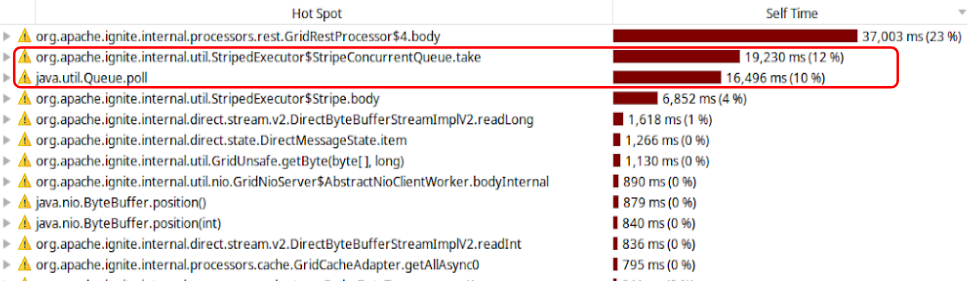
\includegraphics[width=\textwidth]{hotspot.png}
\caption{Hot spot list of Apache Ignite with 30 client threads. The methods are sorted by their total self time, which is : $time\ in\ the\ method - time\ in\ nested\ methods$.}
\label{hotspot}
\end{figure*}

\subsubsection{Idea}
We went into this without any prior knowledge of the system. Our first goal was then to get to know the system, and see whether we could identify a bottleneck from the get go. To do these things, we decided to do a general, coarse-grained benchmarking of the whole system. To be able to identify a bottleneck, we ran several benchmarks while increasing the client load, to see if Ignite could scale.
\subsubsection{Method}
We run Apache Ignite on a GCP compute engine with 60 virtual CPUs. We need this high count of cores to observe the behavior of the system when it is forced to reach a high amount of parallelism. With many cores, the effect of bottlenecks will become more apparent, and easier to identify.

For our benchmarking purposes, we use YCSB \cite{YCSB}. It is a very complete benchmarking framework for key-value stores. It makes available different workloads to apply to our data store. We focus on 3 different workloads : the first one, "A" is write-intensive, with 50\% of update requests and 50\% of reads. The second one, "B" is balanced, with 95\% of reads and 5\% of updates. The third one, "C" has 100\% of reads.
Varying the amount of writes and reads and the amount of clients will allow us to make hypothesis on the source of the bottleneck. 
First, if we notice that when we increase the number of parallel clients, the total number of operations per second starts capping, then it means there probably is a bottleneck. Then, if we notice for example that a bottleneck is only present for the workload A, it means that it is the write operation that is costly. We can then locate more easily the root cause.

\subsubsection{Results}
The results of this first benchmarking are in Fig.~\ref{coarse_grained}.
As you can see, the total throughput, meaning the total number of operations per second for all clients increases when we increase the total number of clients, and it starts capping at around 12 parallel threads. There is in fact a bottleneck in the application.

Another interesting observation is that the 3 different workloads have sensibly the same performances, meaning that the bottleneck is not on the data itself, but rather on the logic of the application, and how it manages client requests.

\subsection{Understanding of the system}
\subsubsection{Idea}
Now that we have identified a bottleneck, the burning question is : why ? How can we find the root cause ?
What we first did is to look at the code of Ignite to understand the logic of the application. Find the entry points and the important data structures, to see where contention could occur.

As explained before, Ignite is a very dense piece of software with a lot of lines of code. To know where to look, we followed the journey of one request and how it is treated by the data store.

\subsubsection{Findings}
This study allowed us to identify the key data structure of the whole application. All the data is stored in a ConcurrentMap. It could be a source of contention.

Unfortunately for our purposes, this map is really well optimized, at it is the most important point in the data store. It is not degradable from what we were able to see, as all the important methods are used. 

Finding another potential source of contention using this manual analysis of the code is not a very good idea : there are too many classes and lines of code in Ignite, such that it would take way too long to find a issue in it if there even is one. 

\subsection{Profiling}
\subsubsection{Idea}
As explained, parsing the code manually is not a good idea. Our next idea is thus to use a tool to identify issues in the software. Precisely, we want to be able to see what objects and methods are taking a lot of time in the execution. Ideally we want to see an object which takes increasingly more time as we increase the load. This would mean that it is the cause of the bottleneck. What we are looking for is a way to see the call stack of the JVM. 

\subsubsection{Method}
We first tried to use the perf linux profiler \cite{perf}, which was able to fetch the call stack of the JVM process, and we then were able to represent this data in a flame graph. Unfortunately, perf is a linux tool, and thus has no access to the inner workings of the JVM. In fact, the only methods perf is able to fetch from the call stack are the just-in-time (JIT) compiled methods. The JIT compilation allows some java methods to behave like native ones by compiling them at runtime. These methods are then recognized by perf just like native ones. Only certain methods with high usage are JIT, such that the data we obtained is incomplete.

To obtain a more complete amount of data, we need to use JVM specific tools. We used namely JProfiler \cite{jprofiler} to profile the JVM during the execution of Ignite. It has many features, but what interests us is the call tree feature : by regularly sampling the JVM call stack, which is a representation of all the methods called at a certain time, we build a tree of methods called in the whole execution and the time taken by each method. A very interesting feature of JProfiler is the hot spots list : it takes the call tree, and sorts the methods by their self time.

The self time is the total time in the method minus the time in the nested methods.

\subsubsection{Results}
The hot spot list of Ignite we obtained for 30 client threads is in Fig.4.

We can see a lot of methods in the list, but a few are very interesting to us.

First of all, as explained before, we are running JProfiler for Ignite with 30 client threads. We know for a fact that with this load, there is a bottleneck, thus we are expecting to see a method taking a considerable amount of time.

The first method we can see that takes a lot of time is GridRestProcessor.body. When looking in the code, we can see that this method is just a starting point for all methods below, and as such, takes up a lot of time, but can't be considered the cause of a bottleneck.

The two methods below however, surrounded by red, are very interesting. They are linked, as the StripeConcurrentQueue.take calls Queue.poll. As you can see, these methods take up to 12\% of the total execution time, which is considerable. Going into the code, we can see that the StripeConcurrentQueue is a data structure supposed to store the requests for them to be processed. The take method is the reading of this queue by the Ignite workers. It is a very interesting object, as it is in a key location for Ignite, at the entry point. It is also a object that seems to have concurrent accesses, and that takes a lot of execution time when there is a high load. As you can see, it is a very promising object for our purposes.

To link this to the bottleneck we noticed prior, we then need to ensure that the time taken by the StripeConcurrentQueue increases when we increase the load. We therefore plotted the portion of time taken by these methods in Fig. 5.

\begin{figure}[!ht]
\centerline{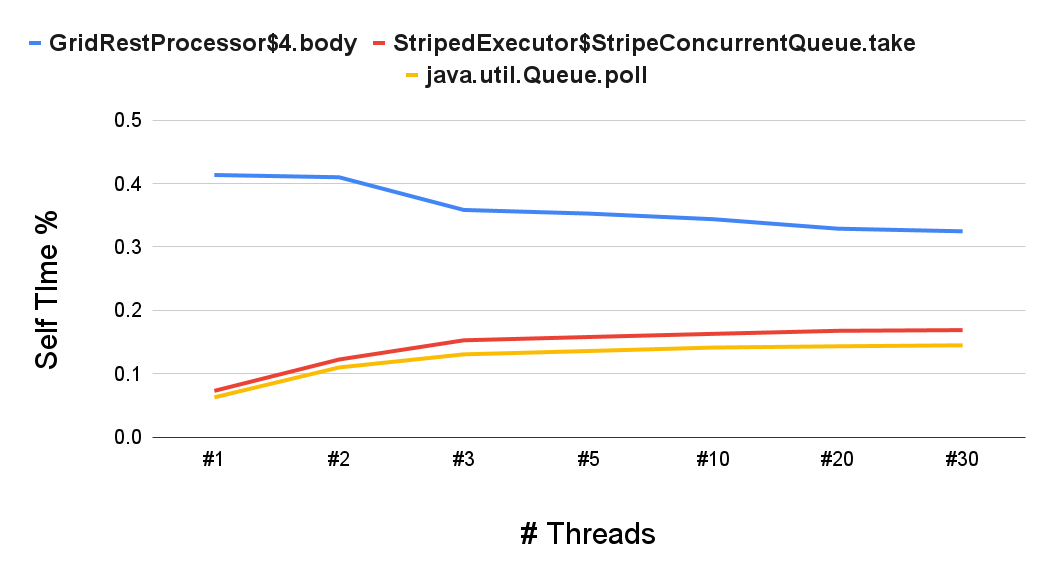
\includegraphics[width=90mm]{selftime.png}}
\caption{Evolution of the time taken by some methods relative to the total time of execution of Apache Ignite when increasing the client load}
\label{selftime}
\end{figure}

As you can see, there is an increase in the time percentage of the take method when we increase the amount of client threads. Unfortunately, JProfiler is a very costly tool, and changes the execution of the program a lot. The way we use it, JProfiler periodically samples the call stack, and sends it via ssh to a remote computer where we treat the data. This introduces a significant overhead. So much so that from the 35000 operations per second we were able to reach prior (Fig.~\ref{coarse_grained}), we now only reach around 7000. We also reach the performance cap quicker, at around 3 client threads. This is why we also see capping in the time percentage of the take method in the graph we plotted. We therefore can't conclude only with profiling, as it is impossible to verify if the bottleneck is in fact caused by it. 

\subsection{Fine-grained Probing}
\subsubsection{Idea}
The prior experiments with JProfiler gave us a hint on where to look : the StripeConcurrentQueue data structure seems to take a lot of CPU time, and is a very important entry point to the whole system. However, JProfiler modifies the execution too much, so much so that it is impossible to make any conclusions on whether the StripeConcurrentQueue is an interesting object to pursue. To get to the bottom of it, we need a lighter, less intrusive way of knowing if it is the source of the bottleneck or not.

\subsubsection{Method}
The solution we landed on, was to manually probe the system, as we already knew were to look in a sense. We therefore put probes to measure the time taken by the StripeConcurrentQueue, and more precisely the Queue poll operation, which we suspect is the issue, as the Queue is the underlying data structure implemented with a \textit{ConcurrentLinkedQueue} from Java.Util.Concurrent.

To avoid introducing more contention, we log the time taken in the method in thread local variables, and gather the data only upon receiving an outside signal, that we manually send to the process when the workload is finished.
\subsubsection{Results}


\begin{figure*}
     \centering
     \begin{subfigure}[b]{0.45\textwidth}
         \centering
         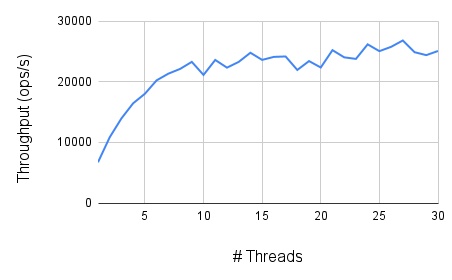
\includegraphics[width=\textwidth]{probe_throughput.png}
         \caption{YCSB workload B of Apache Ignite with probing}
         \label{benchmark_probe}
     \end{subfigure}
     \hfill
     \begin{subfigure}[b]{0.45\textwidth}
         \centering
         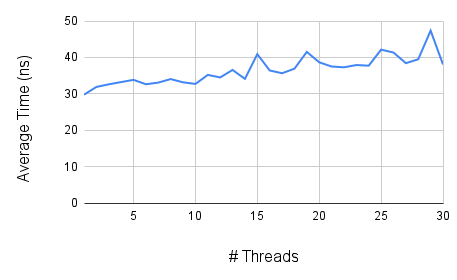
\includegraphics[width=\textwidth]{probe_results.png}
         \caption{Average time in Queue.poll (in ns)}
         \label{avg_poll}
     \end{subfigure}
\caption{Manual probing of Apache Ignite to see the time usage of the Queue.poll method in StripeConcurrentQueue. The two graphs are correlated with a Pearson coefficient of 0.62.}
\label{probe}
\end{figure*}

The results we obtained can be seen in Fig.~\ref{probe}. As you can see in Fig.~\ref{benchmark_probe}, the probing is light enough so that the execution is not modified too much.We reach a throughput that is comparable to the one we reached prior at around 25000 operations/second. This is thanks to our thread local logging of the data we collect to avoid contention.

Fig.~\ref{avg_poll} shows the evolution of the poll method when increasing the client load. As you can see, it clearly increases. Even more so, it is highly correlated with the evolution of the throughput (\textit{i.e} the performance), with a Pearson coefficient \cite{pearson} of $0.62$.
\bigbreak


\section{Going Further}
We were able to expose a correlation between the performances of Apache Ignite, and the time taken by the Queue poll operation. It remains to be seen whether there is a causal relationship between the two. To do so, we would need to modify the poll method to see if there is a change in performance. This is where we come back to the main idea of this project. We should change the ConcurrentLinkedQueue implementation to a degraded one, and observe performance.

Study of the ConcurrentLinkedQueue usage in Ignite shows that it isn't degradable in the first sense of the term, meaning that all key methods of the object are used. Namely, the poll, push and size methods are all used. However, there is another way of degrading a data structure, revolving on the way the object is used.

If an object is used in a asymmetric way, with threads that only do writing and threads that only do reading, and even more, if there only is one reader or one writer to the data structure, we could change the implementation of the object, by alleviating the safety constraints, and thus make it more performant and scalable.

Unfortunately, we hadn't enough time to do this for this project.

If it is discovered that the degradation of the ConcurrentLinkedQueue does not result in better performance, the solution would be going back to profiling Ignite. We were limited with JProfiler during the project as we were using a free trial. If we had had more time, we might have been able to tweak the profiling so that it is less taxing on the system, and thus have better insight on the behavior of Ignite, and where other bottlenecks could be.


\bigbreak
\section{Conclusions}
Our goal was to apply degradable data structures in a modern application such that it had a significant effect on performance.
To do so, we first identified a bottleneck in the data store Apache Ignite, and then proposed a method of identifying the root cause, by first doing a general coarse-grained profiling of the system, and then manually probing the system to remove the overhead caused by profiling. We discovered a candidate to degradation in the form of the ConcurrentLinkedQueue, but hadn't enough time to apply it.


\bigbreak

\section{Acknowledgments}
This project was realised under the supervision of Pierre Sutra, and with the help of Boubacar Kane, whom I would like to both thank dearly, as their advice and guidance was extremely helpful and insightful. 

\bigbreak

\begin{thebibliography}{00}
\bibitem{scalable} \href{https://dl.acm.org/doi/10.1145/2699681}{Austin T. Clements, M. Frans Kaashoek, Nickolai Zeldovich, Robert T. Morris, and Eddie Kohler. 2015. The scalable commutativity rule: Designing scalable software for multicore processors. ACM Trans. Comput. Syst. 32, 4, Article 10 (January 2015), 47 pages.}
\bibitem{degradation} Boubacar Kane, Pierre Sutra. Degradable Objects: A Principled and Efficient Approach to Data Consistency. \textbf{WIP}
\bibitem{ignite} \href{https://ignite.apache.org/docs/latest/}{Apache Ignite}
\bibitem{gcpcompute} \href{https://cloud.google.com/compute/docs}{Google Cloud Platform Compute Engine}
\bibitem{moore} \href{https://ieeexplore.ieee.org/document/591665}{R. R. Schaller, "Moore's law: past, present and future," in IEEE Spectrum, vol. 34, no. 6, pp. 52-59, June 1997, doi: 10.1109/6.591665.}
\bibitem{amdahl} \href{https://conservancy.umn.edu/handle/11299/104341}{Gene M. Amdahl (1989), Oral history interview with Gene M. Amdahl, Charles Babbage Institute, University of Minnesota, hdl:11299/104341.}
\bibitem{java_concurrent} \href{https://docs.oracle.com/javase/8/docs/api/index.html?java/util/concurrent/package-summary.html}{Java.Util.Concurrent}
\bibitem{YCSB} \href{https://ycsb.site}{YCSB}
\bibitem{jprofiler} \href{https://www.ej-technologies.com/products/jprofiler/overview.html}{JProfiler}
\bibitem{perf} \href{https://perf.wiki.kernel.org/index.php/Main_Page}{Perf linux profiler}
\bibitem{pearson} \href{https://libguides.library.kent.edu/SPSS/PearsonCorr}{Pearson Coefficient}
\end{thebibliography}

\vspace{12pt}
\end{document}
